\clearpage

\section{VaLOR 3-flavour oscillation probability calculations}
\label{appendix:valor_3f_osc_prob_code}

In this analysis, 3-flavour neutrino oscillation probabilities in constant density matter are used. Vacuum 3-flavour oscillation 
probabilites are also calculated, but these are used only to estimate the accuracy of the 3-flavour probabilities in matter (see 
section \ref{sec:3flavouraccuracy}). 
The method of calculation of the vacuum probabilities is given in section \ref{sec:vacuumosc}, while the calculation 
of the probabilities in constant density matter is described in section \ref{sec:matterosc}. The code that makes these calculations 
has been integrated into the VaLOR oscillation analysis package. In section \ref{sec:3flavourresults}, 
comparisons are given between 2-flavour and 3-flavour (in matter) oscillation probabilities, and between 3-flavour oscillation probabilities 
in vacuum and matter. Validation of the code is described in section \ref{sec:3flavourvalidation}: the vacuum probabilities were validated 
by comparing their values with those obtained from an alternative formulation in the PDG review. Several validation checks of 
the probabilities in constant density matter are made as they are calculated, and the values of the probabilities were checked 
by comparing them with those given by an independently-written program. Finally, an estimate of the accuracy of the oscillation 
probabilities in matter is given in section \ref{sec:3flavouraccuracy}.
   
\subsection{3-flavour neutrino oscillation probabilities in vacuum}
\label{sec:vacuumosc}

The 3-flavour neutrino oscillation probabilities in vacuum are calculated from equation 11 in \cite{kayser2005}:
\begin{equation}
P(\nu_{\alpha} \rightarrow \nu_{\beta}) = \delta_{\alpha \beta} - 4 \sum_{i>j} Re(U_{\alpha i}^{*} U_{\beta i} U_{\alpha j} U_{\beta j}^{*})
\sin^{2} \left( \frac{\Delta m_{ij}^{2} L}{4E} \right) + 2 \sum_{i>j} Im(U_{\alpha i}^{*} U_{\beta i} U_{\alpha j} U_{\beta j}^{*})
\sin \left(\frac{\Delta m_{ij}^{2} L}{2E} \right)
\label{3flavouroscprobvacuum}
\end{equation}
In equation \ref{3flavouroscprobvacuum}, $\Delta m_{ij}^{2}$ = $m_{j}^{2}$ - $m_{i}^{2}$, L is the distance from the neutrino target 
in Tokai to Super-K (295 km), E is the neutrino energy, and U is the PMNS matrix in vacuum:

\begin{equation}
U = \left(
\begin{array}{ccc}
c_{12}c_{13} & c_{13}s_{12} & s_{13}e^{-i\delta} \\
-c_{23}s_{12} - s_{13}s_{23}c_{12}e^{i\delta} & c_{12}c_{23} - s_{12}s_{13}s_{23}e^{i\delta} & c_{13}s_{23} \\
s_{12}s_{23} - s_{13}c_{12}c_{23}e^{i\delta} & -s_{23}c_{12} - s_{12}c_{23}s_{13}e^{i\delta} & c_{13}c_{23}
\end{array} \right)
\label{PMNSmatrix}
\end{equation}
with $s_{12} = \sin(\theta_{12})$, $c_{12} = \cos(\theta_{12})$, etc. $P(\bar{\nu}_{\alpha} \rightarrow \bar{\nu}_{\beta})$ 
is calculated by changing the sign of the third term in equation \ref{3flavouroscprobvacuum} (this assumes that CPT is 
conserved).

\subsection{3-flavour neutrino oscillation probabilities in constant density matter}
\label{sec:matterosc}
All three neutrino flavours undergo neutral-current interactions with protons, neutrons and electrons in matter. These 
neutral-current interactions have identical amplitudes for all three flavours, and they produce no observable effects on
the probabilities of oscillation between one flavour and another. However the oscillation probabilities are changed by 
coherent forward scattering of electron neutrinos in charged-current interactions with electrons in matter \cite{kayser2005}.

Using natural units with $\hbar$ = c = 1, the time evolution of neutrino flavour states in vacuum is described by the 
Schr\"odinger equation:

\begin{equation}
i \frac{\partial \mathbf{\psi}}{\partial t} = H_{F} \mathbf{\psi} 
\end{equation}
where
\begin{equation}
  \mathbf{\psi} =\left(
\begin{array}{c}
\psi_{e} \\
\psi_{\mu} \\
\psi_{\tau}
\end{array} \right)
\end{equation}
and $H_{F}$ is the effective Hamiltonian in the flavour-state basis
\begin{equation}
H_{F} = \frac{1}{2E} U M U^{\dagger}
\end{equation}
with M defined by
\begin{equation}
M = \left(
\begin{array}{ccc}
0 & 0 & 0 \\
0 & \Delta m_{21}^{2} & 0 \\
0 & 0 & \Delta m_{31}^{2}
\end{array} \right)
\end{equation}
The calculation of oscillation probabilities requires neutrino flight time to be converted to distance travelled, 
and this conversion assumes that neutrinos are highly relativistic. In 
this calculation, $U M U^{\dagger}$ is used for neutrinos, but its complex conjugate is used for antineutrinos. For neutrinos, 
the effects of the charged-current interactions between electron neutrinos and electrons are taken into account by adding the 
potential $2E \sqrt{2} G_{F} N_{e}$ to the real part of the first diagonal element of $U M U^{\dagger}$, where E is the 
neutrino energy, $G_{F}$ is the Fermi coupling constant, and $N_{e}$ is the number density of electrons in matter. For 
antineutrinos, this potential is subtracted from the real part of the first diagonal element of the complex conjugate of 
$U M U^{\dagger}$ (for further details see section 9.2 in \cite{giunti}). 

After the addition or subtraction of this potential, $U M U^{\dagger}$ (or its complex conjugate) is diagonalised. The eigenvalues 
of a Hermitian matrix are always real; they are calculated by solving the (cubic) characteristic equation using the method 
of del Ferro, Tartaglia and Cardano as described in \cite{kopp}. The differences between the eigenvalues are the effective 
mass-squared differences in matter. The eigenvectors are calculated using an algebraic method: one of the components is set 
to be 1.0 (real), and the other two components are calculated using two of the three simultaneous equations in 
$U M U^{\dagger} - \lambda I = 0$, where the $\lambda$ are the eigenvalues. After being normalised, the three eigenvectors 
become the columns of the effective mixing matrix in matter. 

The initial flavour state of the neutrino is represented by a 1$\times$3 column vector whose entries are complex; if, for 
example, the initial flavour state is a muon neutrino, this column vector is 

\begin{displaymath}
\left(
\begin{array}{c}
0 \\
1 \\
0 
\end{array} \right)
\end{displaymath}
The vector representing the initial flavour state is then multiplied by the Hermitian conjugate of the matter mixing matrix 
to convert it to another 1$\times$3 complex column vector representing the initial mass states. These mass states are propagated 
to Super-K by multiplying the jth initial mass state by $\exp \left(\frac{-i \Delta m_{j1}^{2}L}{2E} \right)$, where the 
$\Delta m_{j1}^{2}$ are the mass-squared differences in matter, i.e.\ the differences between the eigenvalues of $U M U^{\dagger}$. 
This gives a new 1$\times$3 complex column vector representing the final mass states, and these are converted to the final flavour 
states by multiplying by the matter mixing matrix. The entries of the resulting 1$\times$3 complex column vector represent the 
amplitudes of each flavour at Super-K, and the corresponding oscillation probabilities are calculated as the moduli squared of these 
amplitudes.  

\subsection{Inputs to the 3-flavour neutrino oscillation probability calculations}

When calculating the 3-flavour oscillation probabilities, the mixing angles can be input either in the form $\sin^{2}(2 \theta_{ij})$ 
or as $\sin^{2}(\theta_{ij})$. $\sin(\theta_{ij})$ and $\cos(\theta_{ij})$ are calculated from the input values, and these are used in 
turn to calculate the elements of $U$. The ``solar'' mass-squared difference is input as $\Delta m_{21}^{2}$, and this is $>$ 0 for 
both mass hierarchies. The ``atmospheric'' 
mass-squared difference is input either as $|\Delta m_{32}^{2}|$ or using a definition introduced by G.\ Fogli, E.\ Lisi et al.\ in 
\cite{LisiGlobalAnalysis}:
\begin{equation}
\Delta m^{2}_{FL} = m_{3}^{2} - \frac{m_{2}^{2} + m_{1}^{2}}{2}
\end{equation}
The quantity denoted $\Delta m^{2}_{FL}$ is useful since its absolute value is the same for both mass hierarchies, and only its sign 
changes. If the atmospheric mass-squared difference is input as $\Delta m^{2}_{32}$, the mass hierarchy is set using the sign of 
$\Delta m_{32}^{2}$; this is positive for the normal mass hierarchy (NH) and negative for the inverted mass hierarchy (IH). In this case, 
$\Delta m_{31}^{2}$ is not input but is calculated as $\Delta m_{31}^{2}$ = $\Delta m_{21}^{2}$ + $\Delta m_{32}^{2}$ for both hierarchies.
If the atmospheric mass-squared difference is input as $\Delta m^{2}_{FL}$, the mass hierarchy is set using the sign of $\Delta m^{2}_{FL}$. 
Then $\Delta m_{32}^{2}$ and $\Delta m_{31}^{2}$ are calculated from the input values of $\Delta m^{2}_{FL}$ and $\Delta m_{21}^{2}$.

\subsection{Results of the 3-flavour neutrino oscillation probability calculations}
\label{sec:3flavourresults}

A comparison of 2-flavour and 3-flavour (in matter) $\nu_{\mu}$-survival probabilities is given in figure \ref{pnumunumucomp}. 
In this figure, the nominal probabilities are calculated with $\sin^{2}(2 \theta_{12})$ = 0.87, $\sin^{2}(2 \theta_{13})$ = 0.1,
$\sin^{2}(2 \theta_{23})$ = 1.0, $\Delta m_{21}^{2}$ = 7.6 $\times 10^{-5}$  eV$^{2}$/c$^{4}$, $|\Delta m_{32}^{2}|$ = 2.32 $\times$ 10$^{-3}$ eV$^{2}$/c$^{4}$,
$\delta_{CP}$ = 0 and Earth crust density = 2.6 g/cm$^{3}$. The bands represent the maximum and minimum 3-flavour probabilities from 4000 random
variations of the non-23 oscillation parameters within their uncertainties at each energy with the same values of $\sin^{2}(2 \theta_{23})$ and
$|\Delta m_{32}^{2}|$ being used. The uncertainties in $\sin^{2}(2 \theta_{12})$ and $\Delta m_{21}^{2}$ are taken from KamLAND combined
with solar experiments \cite{Kamland}, while those in $\sin^{2}(2 \theta_{13})$ are computed as a weighted average of measurements from Daya Bay
\cite{DayaBay} and Reno \cite{Reno}.

The effect of $\sin^{2}(2 \theta_{13})$ on the 3-flavour $\nu_{\mu}$-survival probability in matter 
is shown in figure \ref{pnumunumus13}: there is a small increase in P($\nu_{\mu} \rightarrow \nu_{\mu}$) at all energies as 
$\sin^{2}(2 \theta_{13})$ increases. Also shown in figure \ref{pnumunumudelta} is the effect of $\delta_{CP}$ on the 3-flavour $\nu_{\mu}$-survival 
probability in matter: as $\delta_{CP}$ increases from 0 to $\pi$, P($\nu_{\mu}\rightarrow\nu_{\mu}$) increases above the oscillation 
maximum and decreases below it for the NH, with these changes being reversed for the IH. 
%A similar comparison for P($\nu_{\mu} \rightarrow \nu_{e}$) in matter is given in figure \ref{pnumunuecomp}, and the effect of $\delta_{CP}$ on
%P($\nu_{\mu} \rightarrow \nu_{e}$) in matter is given in figure \ref{pnumunuedelta}. 
The effects of uncertainties in $\sin^{2}(2 \theta_{12})$ and $\Delta m_{21}^{2}$ on the 3-flavour P($\nu_{\mu}\rightarrow\nu_{\mu}$) in matter 
are shown for the NH in table \ref{numuSurvProbEffectError12}. At 0.6 GeV, uncertainties in $\sin^{2}(2 \theta_{12})$ change 
P($\nu_{\mu}\rightarrow\nu_{\mu}$) by $\approx$ 0.00025 and uncertainties in $\Delta m_{21}^{2}$ change it by $\approx$ 0.0001. 

For the NH, the 3-flavour P($\nu_{\mu}\rightarrow\nu_{\mu}$) is increased below the oscillation
maximum and decreased above it compared with the 2-flavour probability, while for the IH these changes are reversed. The oscillation maximum is at
lower energy for the IH than for the NH, and this can be understood more easily by considering the vacuum probabilities. In equation 
\ref{3flavouroscprobvacuum}, the imaginary terms are zero if $\alpha$ = $\beta$, and only the 3 real terms contribute to the vacuum P($\nu_{\mu} \rightarrow \nu_{\mu}$). 
If the atmospheric mass-squared difference is input as $\Delta m^{2}_{32}$, the terms $|U_{\mu 1}|^{2}$, $|U_{\mu 2}|^{2}$, $|U_{\mu 3}|^{2}$, 
$sin^{2} \left( \frac{\Delta m_{21}^{2} L}{4E} \right)$ and sin$^{2} \left( \frac{\Delta m_{32}^{2} L}{4E} \right)$ are identical for the two hierarchies, 
and the only term that changes between them is sin$^{2} \left( \frac{\Delta m_{31}^{2} L}{4E} \right)$. Since $\Delta m_{31}^{2}$ is lower for the 
IH than for the NH, sin$^{2} \left( \frac{\Delta m_{31}^{2} L}{4E} \right)$ has its maximum at a lower energy for the IH than for the NH. The vacuum 
P($\nu_{\mu}\rightarrow\nu_{\mu}$) depends on 1 - 4 $|U_{\mu 1}|^{2}$$|U_{\mu 3}|^{2}$ sin$^{2} \left( \frac{\Delta m_{31}^{2} L}{4E} \right)$, which means that its minimum is 
at a lower energy for the IH than for the NH.     

Referring to the bands in figure \ref{pnumunumucomp}, the highest $\nu_{\mu}$-survival probabilities for the NH are for low values of $\sin^{2}(2 \theta_{12})$, 
high values of $\sin^{2}(2 \theta_{13})$ and $\delta_{CP}$ near $\pi$ above the oscillation maximum, while below the maximum they are for high values of 
$\sin^{2}(2 \theta_{12})$ and $\sin^{2}(2 \theta_{13})$ and $\delta_{CP}$ near 0. For the IH, the highest probabilities 
are for high values of $\sin^{2}(2 \theta_{12})$ and $\sin^{2}(2 \theta_{13})$ and $\delta_{CP}$ near 0 above the oscillation maximum, but 
for low values of $\sin^{2}(2 \theta_{12})$, high values of $\sin^{2}(2 \theta_{13})$ and $\delta_{CP}$ near $\pi$ below it.

Comparisons of $\nu_{\mu}$ oscillation probabilities 
in vacuum and matter are given for the NH in table \ref{numuOscMatterEffectsNH} and for the IH in 
table \ref{numuOscMatterEffectsIH}. At 0.6 GeV, P($\nu_{\mu}\rightarrow\nu_{e}$) is increased by $\approx$ 0.004 and 
P($\nu_{\mu}\rightarrow\nu_{\tau}$) is decreased by $\approx$ 0.004 in matter compared with vacuum for the NH, while for the 
IH the changes are once more reversed. The $\nu_{\mu}$-survival probability is relatively unaffected by the passage of 
$\nu_{\mu}$ through matter, and is changed by only $\approx$ 0.0001 compared with the vacuum probability at 0.6 GeV.

\begin{figure}
\begin{center}
\resizebox{14cm}{!}{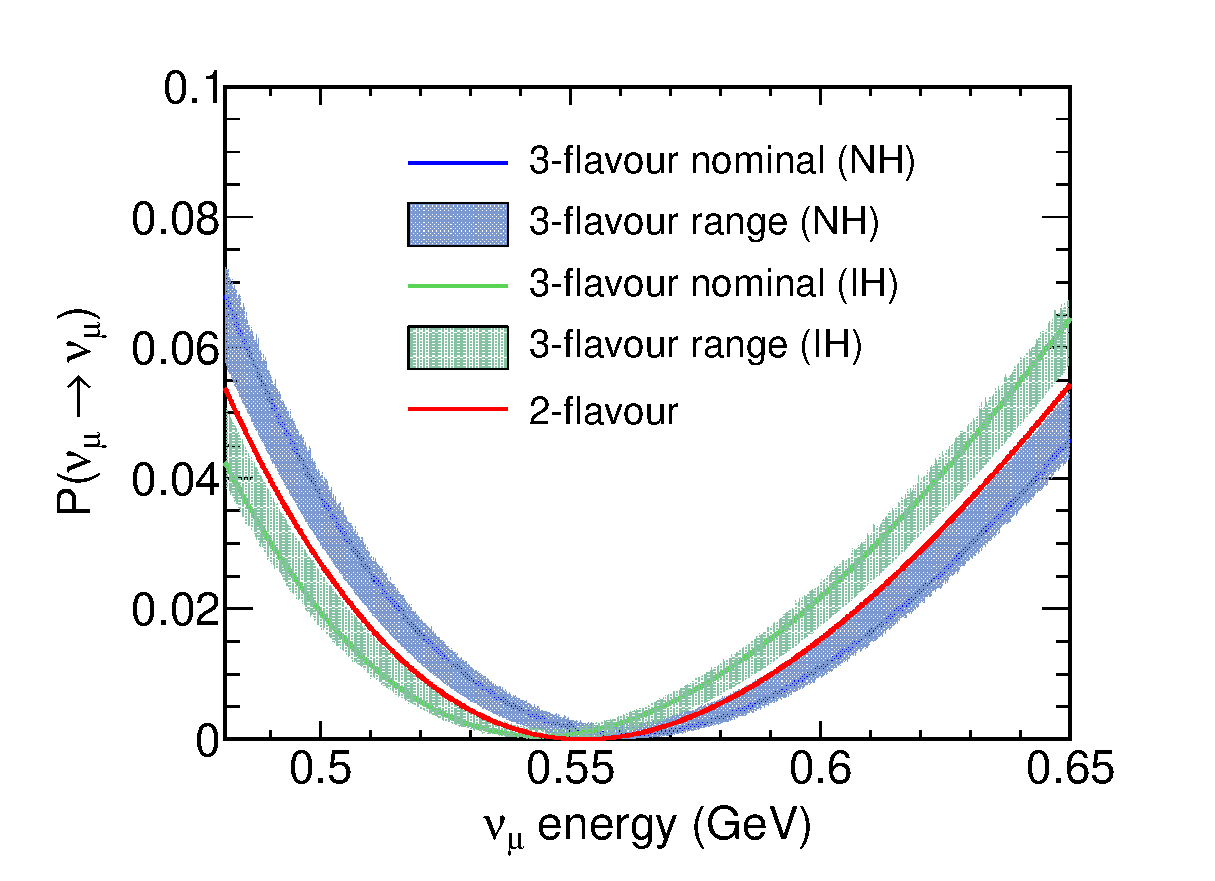
\includegraphics{./images/osc_prob/Prob3NumuSurv.eps}}
\caption[Comparison of P($\nu_{\mu} \rightarrow \nu_{\mu}$) for 2-flavour and 3-flavour (in matter) oscillations]
{Comparison of P($\nu_{\mu} \rightarrow \nu_{\mu}$) for 2-flavour and 3-flavour (in matter) oscillations, NH = normal mass hierarchy,
IH = inverted mass hierarchy. The nominal probabilities are calculated with $\sin^{2}(2 \theta_{12})$ = 0.87, $\sin^{2}(2 \theta_{13})$ = 0.1, 
$\sin^{2}(2 \theta_{23})$ = 1.0, $\Delta m_{21}^{2}$ = 7.6 $\times 10^{-5}$  eV$^{2}$/c$^{4}$, $|\Delta m_{32}^{2}|$ = 2.32 $\times$ 10$^{-3}$ eV$^{2}$/c$^{4}$, 
$\delta_{CP}$ = 0 and Earth crust density = 2.6 g/cm$^{3}$. The bands represent the maximum and minimum 3-flavour probabilities from 4000 random 
variations of the non-23 oscillation parameters within their uncertainties at each energy with the same values of $\sin^{2}(2 \theta_{23})$ and 
$|\Delta m_{32}^{2}|$ being used.}
\label{pnumunumucomp}
\end{center}
\end{figure}

\begin{figure}[ht]
\begin{minipage}[t]{0.48\linewidth}
\centering
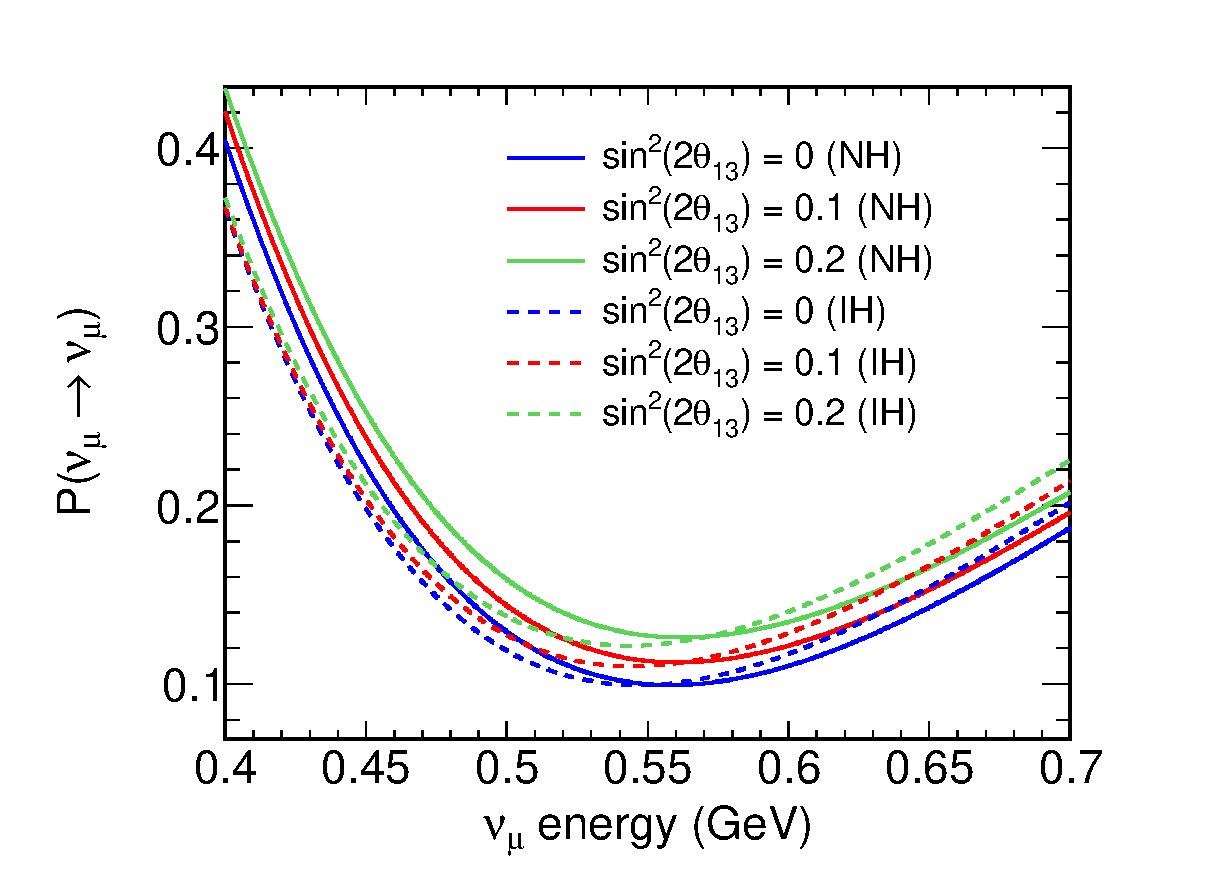
\includegraphics[width=19pc,height=18pc]{./images/osc_prob/Prob3NumuSurvS13.eps}
\caption{
  Effect of $\sin^{2}(2 \theta_{13})$ on P($\nu_{\mu} \rightarrow \nu_{\mu}$) for 3-flavour oscillations in matter; 
  NH = normal mass hierarchy, IH = inverted mass hierarchy, $\sin^{2}(2 \theta_{12})$ = 0.87, $\sin^{2}(2 \theta_{23})$ = 1.0,
  $\Delta m_{21}^{2}$ = 7.6 $\times 10^{-5}$ eV$^{2}$/c$^{4}$, $|\Delta m_{32}^{2}|$ = 2.32 $\times$ 10$^{-3}$ eV$^{2}$/c$^{4}$, $\delta_{CP}$ = 0
  and Earth crust density = 2.6 g/cm$^{3}$.
}
\label{pnumunumus13}
\end{minipage}
\hspace{0.04\linewidth}
\begin{minipage}[t]{0.48\linewidth}
\centering
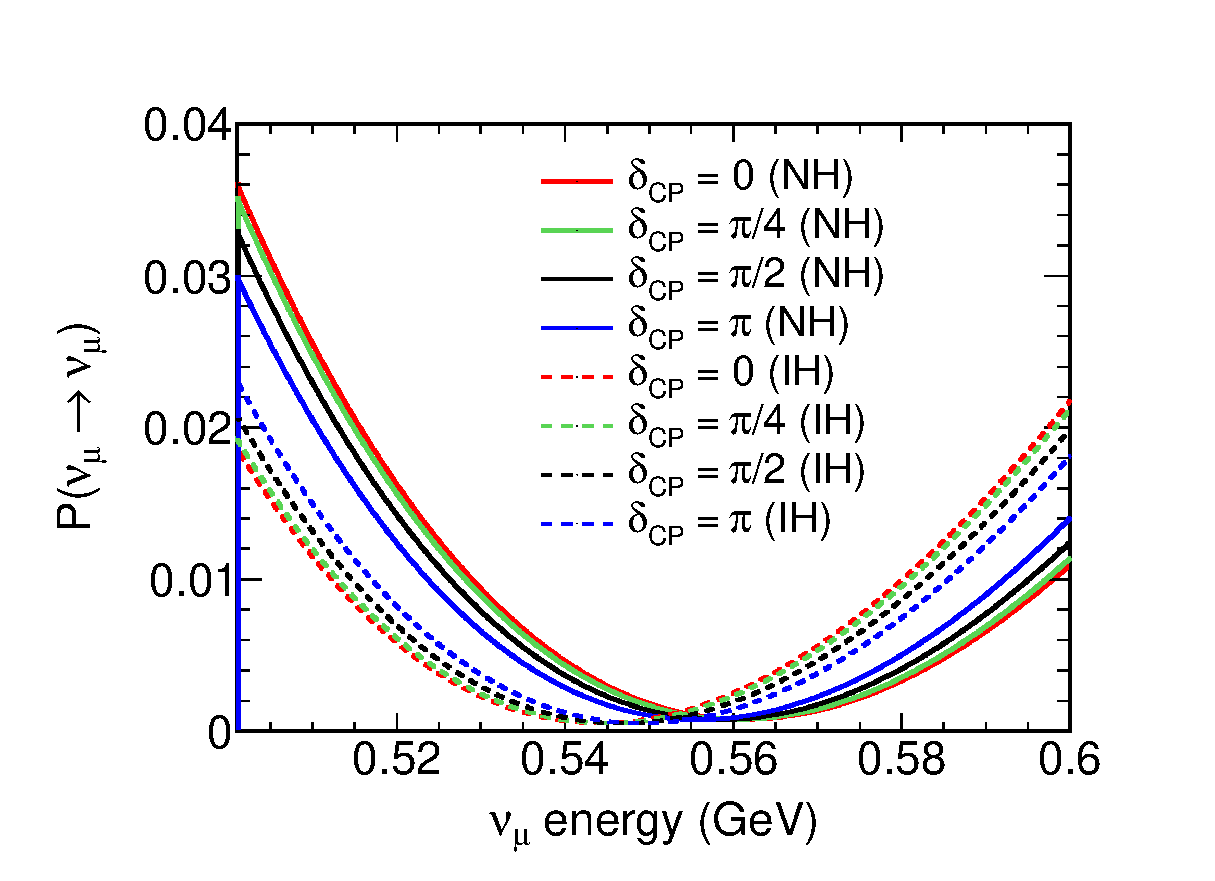
\includegraphics[width=19pc,height=19pc]{./images/osc_prob/Prob3NumuSurvDeltaCP0506.eps}
\caption{
  Effect of $\delta_{CP}$ on P($\nu_{\mu} \rightarrow \nu_{\mu}$) for 3-flavour oscillations in matter; NH = normal mass hierarchy,
  IH = inverted mass hierarchy, $\sin^{2}(2 \theta_{12})$ = 0.87, $\sin^{2}(2 \theta_{13})$ = 0.1, $\sin^{2}(2 \theta_{23})$ = 1.0,
  $\Delta m_{21}^{2}$ = 7.6 $\times 10^{-5}$  eV$^{2}$/c$^{4}$, $|\Delta m_{32}^{2}|$ = 2.32 $\times$ 10$^{-3}$ eV$^{2}$/c$^{4}$ 
  and Earth crust density = 2.6 g/cm$^{3}$.
}
\label{pnumunumudelta}
\end{minipage}
\end{figure}

\begin{table}
\centering
\begin{tabular}{| c | c | c | c | c | c |}
\hline
Energy & P($\nu_{\mu} \rightarrow \nu_{\mu}$) & P($\nu_{\mu} \rightarrow \nu_{\mu}$) &
       P($\nu_{\mu} \rightarrow \nu_{\mu}$) & P($\nu_{\mu} \rightarrow \nu_{\mu}$) & P($\nu_{\mu} \rightarrow \nu_{\mu}$) \\
(GeV) & for $\sin^{2}(2 \theta_{12})$ & for $\sin^{2}(2 \theta_{12})$ & for $\sin^{2}(2 \theta_{12})$
             & for $\sin^{2}(2 \theta_{12})$ & for $\sin^{2}(2 \theta_{12})$ \\
  & = 0.870, & = 0.906, & = 0.833, & = 0.870, & = 0.870, \\
  & $\Delta m_{21}^{2}$ = &  $\Delta m_{21}^{2}$ = & $\Delta m_{21}^{2}$ = & $\Delta m_{21}^{2}$ = & $\Delta m_{21}^{2}$ = \\
  & 7.6 $\times 10^{-5}$  eV$^{2}$/c$^{4}$ & 7.6 $\times 10^{-5}$  eV$^{2}$/c$^{4}$ & 7.6 $\times 10^{-5}$  eV$^{2}$/c$^{4}$ 
   & 7.8 $\times 10^{-5}$ eV$^{2}$/c$^{4}$ & 7.4 $\times 10^{-5}$  eV$^{2}$/c$^{4}$ \\
\hline
0.3 &  0.95703 &  0.95809 &  0.95608 &  0.95733 &  0.95674 \\
\hline
0.4 &  0.35053 &  0.35247 &  0.34877 &  0.35135 &  0.34971 \\
\hline
0.5 &  0.037395 &  0.038009 &  0.036842 &  0.037663 &  0.037129 \\
\hline
0.6 &  0.010963 &  0.010692 &  0.011212 &  0.010841 &  0.011086 \\
\hline
0.7 &  0.094387 &  0.093711 &  0.095004 &  0.094083 &  0.094691 \\
\hline
0.8 &  0.20453 &  0.20371 &  0.20528 &  0.20416 &  0.20490 \\
\hline
0.9 &  0.31099 &  0.31015 &  0.31175 &  0.31061 &  0.31137 \\
\hline
1.0 &  0.40463 &  0.40383 &  0.40535 &  0.40427 &  0.40499 \\
\hline
1.1 &  0.48414 &  0.48340 &  0.48481 &  0.48380 &  0.48447 \\
\hline
1.2 &  0.55080 &  0.55013 &  0.55141 &  0.55050 &  0.55111 \\
\hline
1.3 &  0.60656 &  0.60594 &  0.60711 &  0.60628 &  0.60683 \\
\hline
1.4 &  0.65329 &  0.65274 &  0.65380 &  0.65304 &  0.65354 \\
\hline
1.5 &  0.69265 &  0.69215 &  0.69311 &  0.69243 &  0.69288 \\
\hline
1.6 &  0.72599 &  0.72554 &  0.72640 &  0.72579 &  0.72620 \\
\hline
1.7 &  0.75440 &  0.75399 &  0.75478 &  0.75421 &  0.75459 \\
\hline
1.8 &  0.77876 &  0.77839 &  0.77910 &  0.77859 &  0.77893 \\
\hline
1.9 &  0.79978 &  0.79943 &  0.80009 &  0.79962 &  0.79993 \\
\hline
2.0 &  0.81801 &  0.81770 &  0.81830 &  0.81787 &  0.81815 \\
\hline
\end{tabular}
\caption{
  Effects of uncertainties in $\sin^{2}(2 \theta_{12})$ and $\Delta m_{21}^{2}$ 
  on the 3-flavour P($\nu_{\mu} \rightarrow \nu_{\mu}$) in matter; this is for the normal mass hierarchy, $\sin^{2}(2 \theta_{23})$ = 1.0, 
  $|\Delta m_{32}^{2}|$ = 2.32 $\times$ 10$^{-3}$ eV$^{2}$/c$^{4}$, $\sin^{2}(2 \theta_{13})$ = 0.1 and $\delta_{CP}$ = 0.
}
\label{numuSurvProbEffectError12}
\end{table}

\clearpage

\begin{table}
\centering
\begin{tabular}{| c | c | c | c | c | c | c |}
\hline
Energy (GeV) & \multicolumn{2}{|c|}{P($\nu_{\mu} \rightarrow \nu_{e}$)} & \multicolumn{2}{|c|}{P($\nu_{\mu} \rightarrow \nu_{\mu}$)} & \multicolumn{2}{|c|}{P($\nu_{\mu} \rightarrow \nu_{\tau}$)}\\
\hline
 & Vacuum & Matter & Vacuum & Matter & Vacuum & Matter \\
\hline
0.3 &  0.00054403 &  0.00016981 &  0.95496 &  0.95703 &  0.044501 &  0.042796\\
\hline
0.4 &  0.024253 &  0.029051 &  0.34954 &  0.35053 &  0.62621 &  0.62042\\
\hline
0.5 &  0.046291 &  0.051402 &  0.037071 &  0.037395 &  0.91664 &  0.91120\\
\hline
0.6 &  0.051975 &  0.056108 &  0.010883 &  0.010963 &  0.93714 &  0.93293\\
\hline
0.7 &  0.049739 &  0.052871 &  0.094385 &  0.094387 &  0.85588 &  0.85274\\
\hline
0.8 &  0.044830 &  0.047181 &  0.20455 &  0.20453 &  0.75062 &  0.74829\\
\hline
0.9 &  0.039478 &  0.041256 &  0.31101 &  0.31099 &  0.64951 &  0.64776\\
\hline
1.0 &  0.034502 &  0.035865 &  0.40464 &  0.40463 &  0.56085 &  0.55951\\
\hline
1.1 &  0.030139 &  0.031200 &  0.48415 &  0.48414 &  0.48571 &  0.48466\\
\hline
1.2 &  0.026403 &  0.027241 &  0.55081 &  0.55080 &  0.42279 &  0.42196\\
\hline
1.3 &  0.023233 &  0.023905 &  0.60656 &  0.60656 &  0.37021 &  0.36954\\
\hline
1.4 &  0.020548 &  0.021093 &  0.65329 &  0.65329 &  0.32616 &  0.32562\\
\hline
1.5 &  0.018268 &  0.018715 &  0.69266 &  0.69266 &  0.28908 &  0.28863\\
\hline
1.6 &  0.016325 &  0.016696 &  0.72599 &  0.72599 &  0.25769 &  0.25731\\
\hline
1.7 &  0.014661 &  0.014971 &  0.75440 &  0.75440 &  0.23094 &  0.23063\\
\hline
1.8 &  0.013228 &  0.013491 &  0.77876 &  0.77876 &  0.20801 &  0.20775\\
\hline
1.9 &  0.011988 &  0.012211 &  0.79977 &  0.79978 &  0.18824 &  0.18801\\
\hline
2.0 &  0.010908 &  0.011100 &  0.81801 &  0.81801 &  0.17108 &  0.17089\\
\hline
\end{tabular}
\caption{
 Comparison of $\nu_{\mu}$ oscillation probabilities in vacuum and matter for the normal mass hierarchy, Earth crust
 density = 2.6 g/cm$^{3}$, $ \sin^{2}(2 \theta_{12})$ = 0.87, $\sin^{2}(2 \theta_{13})$ = 0.1, $\sin^{2}(2 \theta_{23})$ = 1.0, 
 $\Delta m_{21}^{2}$ = 7.6 $\times$ 10$^{-5}$ eV$^{2}$/c$^{4}$, $|\Delta m_{32}^{2}|$ = 2.32 $\times$ 10$^{-3}$ eV$^{2}$/c$^{4}$ 
 and $\delta_{CP}$ = 0.
}
\label{numuOscMatterEffectsNH}
\end{table}

\begin{table}
\centering
\begin{tabular}{| c | c | c | c | c | c | c |}
\hline
Energy (GeV) & \multicolumn{2}{|c|}{P($\nu_{\mu} \rightarrow \nu_{e}$)} & \multicolumn{2}{|c|}{P($\nu_{\mu} \rightarrow \nu_{\mu}$)} & \multicolumn{2}{|c|}{P($\nu_{\mu} \rightarrow \nu_{\tau}$)}\\
\hline
 & Vacuum & Matter & Vacuum & Matter & Vacuum & Matter \\
\hline
0.3 &  0.016651 &  0.012718 &  0.91243 &  0.91427 &  0.070915 &  0.073016\\
\hline
0.4 &  0.047961 &  0.041880 &  0.28695 &  0.28747 &  0.66509 &  0.67065\\
\hline
0.5 &   0.052910 &  0.047892 &  0.019598 &   0.019587 &  0.92749 &  0.93252\\
\hline
0.6 &  0.047803 &  0.044104 &  0.021900 &  0.021756 &  0.93030 &  0.93414\\
\hline
0.7 &  0.040787 &  0.038101 &  0.11802 &   0.11787 &  0.84120 &  0.84403\\
\hline
0.8 &  0.034297 &  0.032325 &  0.23236 &  0.23222 &  0.73335 &  0.73545\\
\hline
0.9 &  0.028857 &  0.027381 &  0.33905 &  0.33895 &  0.63210 &  0.63367\\
\hline
1.0 &  0.024433 &  0.023306 &  0.43123 &  0.43115 &  0.54434 &  0.54555\\
\hline
1.1 &  0.020858 &  0.019980 &  0.50865 &  0.50859 &  0.47049 &  0.47143\\
\hline
1.2 &  0.017960 &  0.017265 &  0.57310 &  0.57305 &  0.40894 &  0.40969\\
\hline
1.3 &  0.015595 &  0.015037 &  0.62672 &  0.62669 &  0.35768 &  0.35828\\
\hline
1.4 &  0.013649 &  0.013194 &  0.67151 &  0.67148 &  0.31485 &  0.31533\\
\hline
1.5 &  0.012034 &  0.011657 &  0.70911 &  0.70909 &  0.27886 &  0.27926\\
\hline
1.6 &  0.010681 &  0.010366 &  0.74089 &  0.74087 &  0.24843 &  0.24876\\
\hline
1.7 &  0.0095379 &  0.0092726 &  0.76792 & 0.76791 &  0.22254 &  0.22282\\
\hline
1.8 &  0.0085654 &  0.0083395 &  0.79107 &  0.79105 &  0.20037 &  0.20061\\
\hline
1.9 &   0.0077316 &  0.0075376 &  0.81101 &  0.81010 &  0.18126 &  0.18146\\
\hline
2.0 &  0.0070119 &  0.0068441 &  0.82829 &  0.82829 &  0.16470 &  0.16487\\
\hline
\end{tabular}
\caption
{
  Comparison of $\nu_{\mu}$ oscillation probabilities in vacuum and matter for the inverted mass hierarchy, Earth crust
  density = 2.6 g/cm$^{3}$, $ \sin^{2}(2 \theta_{12})$ = 0.87, $\sin^{2}(2 \theta_{13})$ = 0.1, $\sin^{2}(2 \theta_{23})$ = 1.0,
  $\Delta m_{21}^{2}$ = 7.6 $\times$ 10$^{-5}$ eV$^{2}$/c$^{4}$, $|\Delta m_{32}^{2}|$ = 2.32 $\times$ 10$^{-3}$ eV$^{2}$/c$^{4}$ and $\delta_{CP}$ = 0.
}
\label{numuOscMatterEffectsIH}
\end{table}

\clearpage

\subsection{Validation of the 3-flavour oscillation probabilities}
\label{sec:3flavourvalidation}

The 3-flavour oscillation probabilities in vacuum were checked using an alternative formulation in equations 13.13 and 13.14 
in the PDG review \cite{PDG2012}:
\begin{equation}
P(\nu_{\alpha} \rightarrow \nu_{\beta}) = \sum_{j} |U_{\beta j}|^{2} |U_{\alpha j}|^{2} + 2 \sum_{j>k} |U_{\beta j} U_{\alpha j}^{*} U_{\alpha k} U_{\beta k}^{*}| 
\cos \left(\frac{\Delta m_{jk}^{2} L}{2E}  - \phi_{\beta \alpha;jk}  \right)
\label{3flavouroscprobvacuumpdg}
\end{equation}
where $\phi_{\beta \alpha;jk}$ = arg($U_{\beta j} U_{\alpha j}^{*} U_{\alpha k} U_{\beta k}^{*}$). $P(\bar{\nu}_{\alpha} \rightarrow \bar{\nu}_{\beta})$ 
is calculated by changing the sign of $\phi_{\beta \alpha;jk}$ in the argument of the cosine. The probabilities calculated from equation \ref{3flavouroscprobvacuumpdg} 
agreed with those calculated from equation \ref{3flavouroscprobvacuum} to 14 significant figures.

Several checks of the oscillation probabilities in constant density matter are written into the code that calculates them: 
\begin{enumerate}
\item The eigenvalues of $U M U^{\dagger}$ are checked by comparing their sum with the trace of the matrix. 
\item Each normalised eigenvector is multiplied in turn by each of the 3 matrices formed by subtracting the eigenvalues from the real parts of the 
diagonal elements of $U M U^{\dagger}$, and a check is made of the differences between these products and a zero vector. 
\item A check is made that the normalised eigenvectors of $U M U^{\dagger}$ are orthogonal by calculating the scalar product between them (the scalar product of two 
complex vectors is the product of the first vector with the complex conjugate of the second vector). 
\item A check is also made that the Hermitian conjugate of the mixing matrix in matter is equal to the inverse of the matrix. This is done by multiplying the 
mixing matrix in matter by its Hermitian conjugate, and checking the differences between the product and an identity matrix.
\end{enumerate}

The values of the oscillation probabilities in constant density matter were checked by comparing them with equivalent probabilities calculated by an 
independently-written Fortran program \cite{sloan}. This Fortran program uses different algorithms, and calculates numerically the eigenvalues and 
eigenvectors of $U M U^{\dagger}$. Nevertheless there was very good agreement between the two calculations of the probabilities, with the 
fractional differences being $\approx 2 \times 10^{-6}$. 

The values of the matter oscillation probabilities were also compared with those given by Prob3++ \cite{Prob3}, and the fractional differences were 
$\approx$ 1-5 $\times$ 10$^{-4}$. The comparison plots can be seen in the next Appendix.

\subsection{Accuracy of the 3-flavour oscillation probabilities} 
\label{sec:3flavouraccuracy}

As stated in section \ref{sec:3flavourvalidation}, the 3-flavour oscillation probabilities in vacuum agreed to 14 significant figures between the two 
formulations.

An estimate of the accuracy of the 3-flavour oscillation probabilities in constant density matter was made in three separate ways: 
\begin{enumerate}
\item The matter probabilities for zero density were compared with the vacuum probabilities; there was good agreement, with the fractional differences being 
$\approx$ 2-5 $\times$ 10$^{-6}$. 
\item The probabilites given when calculating the eigenvectors with simultaneous equations 1 and 2 in $U M U^{\dagger} - \lambda I = 0$ were compared 
with the probabilities given when calculating the eigenvectors with simultaneous equations 2 and 3. The fractional differences between these two 
calculations were again $\approx$ 2-5 $\times$ 10$^{-6}$.
\item The sum of three matter probabilities, for example P($\nu_{\mu} \rightarrow \nu_{e}$) + P($\nu_{\mu} \rightarrow \nu_{\mu}$) + 
P($\nu_{\mu} \rightarrow \nu_{\tau}$), was compared with 1.0; again there was good agreement, and the differences were $\approx 2 \times 10^{-6}$. 
\end{enumerate}

This means that the matter oscillation probabilities should be considered to be accurate to 5 decimal places. The accuracy of the matter probabilities 
is less than that of the vacuum probabilities due to the method of calculation of the eigenvectors. This involves calculations of the form 
\begin{displaymath}
\frac{(ab - cd)}{(ef - gh)}
\end{displaymath} 
where a, b, c, etc.\ are elements of $U M U^{\dagger} - \lambda I$. Frequently ab is close in value to cd, which means that (ab - cd) is much smaller than ab or 
cd, and the same applies to (ef - gh). However the advantage of the method of calculation of the eigenvectors described in section \ref{sec:matterosc} 
is that it allows  the worst of these cancellation errors to be avoided; this can be done by calculating the eigenvectors using different pairs of 
simultaneous equations in  $U M U^{\dagger} - \lambda I = 0$ for different combinations of the oscillation parameters. 
In practice, the eigenvectors are nearly always calculated using equations 1 and 2 in $U M U^{\dagger} - \lambda I = 0$, 
but equations 2 and 3 are used when 3.10 $<$ $\delta_{CP}$ $<$ 3.18 and 
$\sin^{2}(2 \theta_{13})$ $>$ $10^{-8}$ in order to avoid such cancellation errors.  







